\setcounter{section}{0}
\section{GIÁ TRỊ LƯỢNG GIÁC}
\subsection{Giá trị lượng giác của góc lượng giác}
\begin{bt}%[Lê Minh Thiện Anh, dự án 11SGK-KNTT-2022]%[1K1Y1-1]
	Hoàn thành bảng sau
	\begin{center}
	\renewcommand{\arraystretch}{2}
	\begin{tabular}{|c|c|c|c|c|c|l|}
	\hline
	Số đo độ     & $15^\circ$ & ? & $0^\circ$ & $900^\circ$ & ? & ?  \\ \hline
	Số đo radian & ?  & $\dfrac{3\pi}{8}$ & ? & ?   & $-\dfrac{7\pi}{12}$ & $-\dfrac{11\pi}{8}$ \\ \hline
	\end{tabular}
	\end{center}
	\loigiai{
		\begin{center}
		\renewcommand{\arraystretch}{2}
		\begin{tabular}{|c|c|c|c|c|c|l|}
		\hline
		Số đo độ     & $15^\circ$ & $\left(\dfrac{135}{2}\right)^\circ$ & $0^\circ$ & $900^\circ$ & $-105^\circ$ & $-\left(\dfrac{495}{2}\right)^\circ$  \\ \hline
		Số đo radian & $\dfrac{\pi}{12}$  & $\dfrac{3\pi}{8}$ & $0$ & $5\pi$   & $-\dfrac{7\pi}{12}$ & $-\dfrac{11\pi}{8}$ \\ \hline
		\end{tabular}
		\end{center}
}
\end{bt}

\begin{bt}%[Lê Minh Thiện Anh, dự án 11SGK-KNTT-2022]%[1K1Y1-3]
	Một đường tròn có bán kính $20$ cm. Tìm độ dài các cung trên đường tròn đó có số đo sau:
	\begin{multicols}{4}
		\begin{enumerate}
			\item $\dfrac{\pi}{12}$;
			\item $1{,}5$;
			\item $35^\circ$;
			\item $315^\circ$.
		\end{enumerate}
	\end{multicols}
	\loigiai{
		\begin{enumerate}
			\item $l=R\alpha=20\cdot\dfrac{\pi}{12}=\dfrac{5\pi}{3}$ cm;
			\item $l=R\alpha=20\cdot1{,}5=30$ cm;
			\item Đổi $35^{\circ}=35 \cdot \dfrac{\pi}{180}=\dfrac{7\pi}{36} \mathrm{rad}$.\\
			      Độ dài cung tròn là  $l=R\alpha=20\cdot\dfrac{7\pi}{36}=\dfrac{35\pi}{9}$ cm;
			\item Đổi $315^{\circ}=315 \cdot \dfrac{\pi}{180}=\dfrac{7\pi}{4} \mathrm{rad}$.\\
			      Độ dài cung tròn là  $l=R\alpha=20\cdot\dfrac{7\pi}{4}=35$ cm.
		\end{enumerate}
	}
\end{bt}

\begin{bt}%[Lê Minh Thiện Anh, dự án 11SGK-KNTT-2022]%[1K1Y1-4]
	Trên đường tròn lượng giác, xác định điểm $M$ biểu diễn các góc lượng giác có số đo sau:
	\begin{multicols}{4}
		\begin{enumerate}
			\item $\dfrac{2\pi}{3}$;
			\item $-\dfrac{11\pi}{4}$;
			\item $150^\circ$;
			\item $-225^\circ$.
		\end{enumerate}
	\end{multicols}
	\loigiai{
		\begin{enumerate}
			\item Điểm $M$ trên đường đường tròn lượng giác biểu diễn góc lượng giác có số đo bằng $\dfrac{2\pi}{3}$ được xác định trong hình sau
			      \begin{center}
				      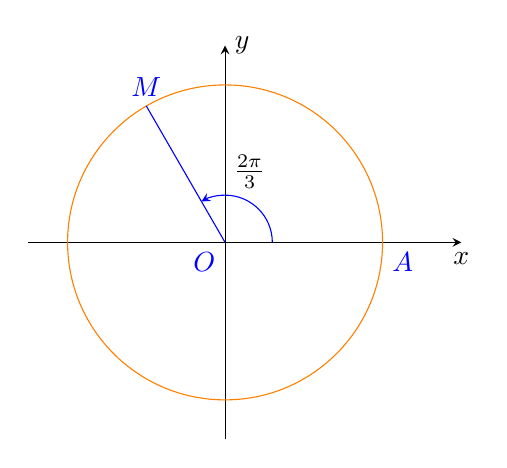
\begin{tikzpicture}
					      \draw[-stealth] (-2.5,0) -- (3,0)node[below] {$x$};
					      \draw[-stealth] (0,-2.5) -- (0,2.5)node[right] {$y$};
					      \draw[orange] (0,0) circle (2);
					      \draw[-stealth,blue] (0:.6) arc (0:120:.6);
					      \draw[blue] (0:0) node[below left]{$O$}--(120:2) node[above]{$M$};
					      \path (75:1.2) node[below=-2pt]{$\frac{2\pi}{3}$};
					      \path (0:2) node[below right,blue]{$A$};
				      \end{tikzpicture}
			      \end{center}
			\item Điểm $M$ trên đường đường tròn lượng giác biểu diễn góc lượng giác có số đo bằng $-\dfrac{11\pi}{4}$ được xác định trong hình sau
			      \begin{center}
				      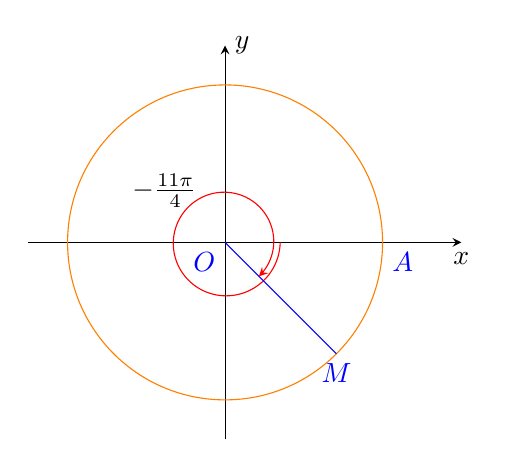
\begin{tikzpicture}
					      \draw[-stealth] (-2.5,0) -- (3,0)node[below] {$x$};
					      \draw[-stealth] (0,-2.5) -- (0,2.5)node[right] {$y$};
					      \draw[orange] (0,0) circle (2);
					      \draw[red,-stealth,smooth,samples=100] plot[domain =0:-2.25*pi]({.7*(1.02)^(\x) *cos(\x r)},{.7*(1.02)^(\x) *sin(\x r)});
					      \draw[blue] (0:0) node[below left]{$O$}--(-45:2) node[below]{$M$};
					      \path (130:1.2) node[below=-2pt]{$-\frac{11\pi}{4}$};
					      \path (0:2) node[below right,blue]{$A$};
				      \end{tikzpicture}
			      \end{center}
			\item Điểm $M$ trên đường đường tròn lượng giác biểu diễn góc lượng giác có số đo bằng $150^{\circ}$ được xác định trong hình sau
			      \begin{center}
				      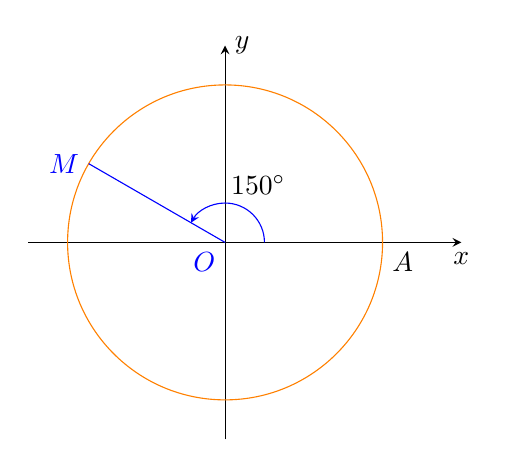
\begin{tikzpicture}
					      \draw[-stealth] (-2.5,0) -- (3,0)node[below] {$x$};
					      \draw[-stealth] (0,-2.5) -- (0,2.5)node[right] {$y$};
					      \draw[orange] (0,0) circle (2);
					      \draw[-stealth,blue] (0:.5) arc (0:150:.5);
					      \draw[blue] (0:0) node[below left]{$O$}--(150:2) node[left]{$M$};
					      \path (65:1) node[below=-2pt]{$150^{\circ}$};
					      \path (0:2) node[below right]{$A$};
				      \end{tikzpicture}
			      \end{center}
			\item Điểm $M$ trên đường đường tròn lượng giác biểu diễn góc lượng giác có số đo bằng $-225^{\circ}$ được xác định trong hình sau
			      \begin{center}
				      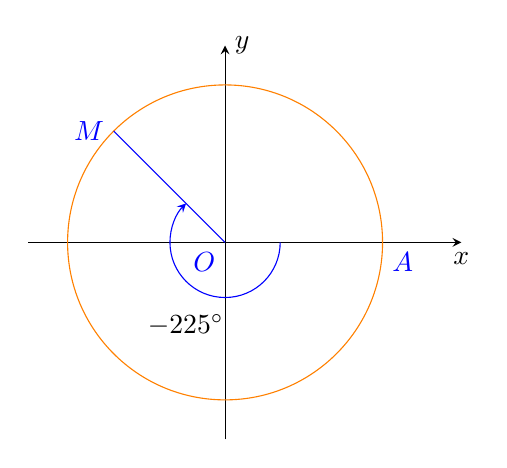
\begin{tikzpicture}
					      \draw[-stealth] (-2.5,0) -- (3,0)node[below] {$x$};
					      \draw[-stealth] (0,-2.5) -- (0,2.5)node[right] {$y$};
					      \draw[orange] (0,0) circle (2);
					      \draw[-stealth,blue] (0:.7) arc (0:-225:.7);
					      \draw[blue] (0:0) node[below left]{$O$}--(-225:2) node[left]{$M$};
					      \path (-120:1) node[below=-2pt]{$-225^{\circ}$};
					      \path (0:2) node[below right,blue]{$A$};
				      \end{tikzpicture}
			      \end{center}
		\end{enumerate}
	}
\end{bt}

\begin{bt}%[Lê Minh Thiện Anh, dự án 11SGK-KNTT-2022]%[1K1B1-6]
	Tính các giá trị lượng giác của góc $\alpha$, biết
	\begin{enumerate}
		\item $\cos\alpha=\dfrac{1}{5}$ và $0<\alpha<\dfrac{\pi}{2}$;
		\item $\sin\alpha=\dfrac{2}{5}$ và $\dfrac{\pi}{2}<\alpha<\pi$;
		\item $\tan\alpha=\sqrt{5}$ và $\pi<\alpha<\dfrac{3\pi}{2}$;
		\item $\cot\alpha=-\dfrac{1}{\sqrt{2}}$ và $\dfrac{3\pi}{2}<\alpha<2\pi$.
	\end{enumerate}
	\loigiai{
		\begin{enumerate}
			\item Ta có $\sin^2\alpha+\cos^2\alpha=1\Rightarrow \sin^2\alpha=1-\cos^2\alpha\Leftrightarrow \hoac{& \sin\alpha=\sqrt{1-\cos^2\alpha}\\&\sin\alpha=-\sqrt{1-\cos^2\alpha}.}$\\
			      Vì $0<\alpha<\dfrac{\pi}{2}$ nên $\sin\alpha>0$, suy ra $\sin\alpha=\sqrt{1-\cos^2\alpha}$\\
			      $\Rightarrow\sin\alpha=\sqrt{1-\left(\dfrac{1}{5}\right)^2}=\sqrt{\dfrac{24}{25}}=\dfrac{2\sqrt{6}}{5}$.\\
			      Mà $\tan\alpha=\dfrac{\sin\alpha}{\cos\alpha}$ nên $\tan\alpha=\dfrac{2\sqrt{6}}{5}:\dfrac{1}{5}=2\sqrt{6}$ và $\cot\alpha=\dfrac{\sqrt{6}}{12}$.
			\item Ta có $\sin^2\alpha+\cos^2\alpha=1\Rightarrow \cos^2\alpha=1-\sin^2\alpha\Leftrightarrow \hoac{& \cos\alpha=\sqrt{1-\sin^2\alpha}\\&\cos\alpha=-\sqrt{1-\sin^2\alpha}.}$\\
			      Vì $\dfrac{\pi}{2}<\alpha<\pi$ nên $\cos\alpha<0$, suy ra $\cos\alpha=-\sqrt{1-\sin^2\alpha}$\\
			      $\Rightarrow\cos\alpha=-\sqrt{1-\left(\dfrac{2}{5}\right)^2}=-\sqrt{\dfrac{21}{25}}=-\dfrac{\sqrt{21}}{5}$.\\
			      Mà $\tan\alpha=\dfrac{\sin\alpha}{\cos\alpha}$ nên $\tan\alpha=\dfrac{2}{5}:\left(-\dfrac{\sqrt{21}}{5}\right)=-\dfrac{2\sqrt{21}}{21}$ và $\cot\alpha=-\dfrac{\sqrt{21}}{2}$.
			\item Vì $\pi<\alpha<\dfrac{3\pi}{2}$ nên $\cos\alpha<0$, do đó từ công thức:\\
			      $1+\tan^2\alpha=\dfrac{1}{\cos^2\alpha}$, suy ra $\cos^2\alpha=\dfrac{1}{1+\tan^2\alpha}$.\\
			      $\Rightarrow\cos\alpha=-\dfrac{1}{\sqrt{1+\tan^2\alpha}}=-\dfrac{1}{\sqrt{1+(\sqrt{5})^2}}=-\dfrac{\sqrt{6}}{6}$;\\ $\cot\alpha=\dfrac{1}{\tan\alpha}=\dfrac{\sqrt{5}}{5}$ và $\sin\alpha=\tan\alpha\cdot\cos\alpha=-\dfrac{\sqrt{30}}{6}$.
			\item
			      Vì $\dfrac{3\pi}{2}<\alpha<2\pi$ nên $\sin\alpha<0$, do đó từ công thức:\\
			      $1+\cot^2\alpha=\dfrac{1}{\sin^2\alpha}$, suy ra $\sin^2\alpha=\dfrac{1}{1+\cot^2\alpha}$.\\
			      $\Rightarrow\sin\alpha=-\dfrac{1}{\sqrt{1+\cot^2\alpha}}=-\dfrac{1}{\sqrt{1+\left(-\dfrac{1}{\sqrt{2}}\right)^2}}=-\dfrac{\sqrt{6}}{3}$;\\ $\tan\alpha=\dfrac{1}{\cot\alpha}=-\sqrt{2}$ và $\cos\alpha=\cot\alpha\cdot\sin\alpha=\dfrac{\sqrt{3}}{3}$.
		\end{enumerate}
	}
\end{bt}

\begin{bt}%[Lê Minh Thiện Anh, dự án 11SGK-KNTT-2022]%[1K1B1-8]
	Chứng minh các đẳng thức:
	\begin{enumerate}
		\item $\cos^4\alpha-\sin^4\alpha=2\cos^2\alpha-1$;
		\item $\dfrac{\cos^2\alpha+\tan^2\alpha-1}{\sin^2\alpha}=\tan^2\alpha$.
	\end{enumerate}
	\loigiai{
		\begin{enumerate}
			\item Ta có
			      \begin{eqnarray*}
				      \cos^4\alpha-\sin^4\alpha&=& \left(\cos^2\alpha-\sin^2\alpha\right)\left(\cos^2\alpha+\sin^2\alpha\right)\\
				      &= & \cos^2\alpha-\left(1-\sin^2\alpha\right)\\
				      &= & 2\cos^2\alpha-1.
			      \end{eqnarray*}
			\item Ta có
			      \begin{eqnarray*}
				      \dfrac{\cos^2\alpha+\tan^2\alpha-1}{\sin^2\alpha}&=& \dfrac{\cos^2\alpha-1}{\sin^2\alpha}+\dfrac{\tan^2\alpha}{\sin^2\alpha}\\
				      &= & \dfrac{-\sin^2\alpha}{\sin^2\alpha}+\dfrac{\sin^2\alpha}{\cos^2\alpha}\cdot\dfrac{1}{\sin^2\alpha}\\
				      &= & \dfrac{1}{\cos^2\alpha}-1\\
				      &=&\dfrac{1-\cos^2\alpha}{\cos^2\alpha}\\
				      &=&\dfrac{\sin^2\alpha}{\cos^2\alpha}=\tan^2\alpha.
			      \end{eqnarray*}
		\end{enumerate}
	}
\end{bt}

\begin{bt}%[Lê Minh Thiện Anh, dự án 11SGK-KNTT-2022]%[1K1B1-9]
	Bánh xe của người đi xe đạp quay được $11$ vòng trong $5$ giây.
	\begin{enumerate}
		\item Tính góc (theo độ và theo radian) mà bánh xe quay được trong $1$ giây;
		\item Tính độ dài quãng đường mà người đi xe đã đi được trong $1$ phút, biết rằng đường kính của xe đạp là $680$ mm.
	\end{enumerate}
	\loigiai{
		\begin{enumerate}
			\item Trong $1$ giây, bánh xe quay được $\dfrac{11}{5}$ (vòng).\\
			      Vì $1$ vòng ứng với $360^\circ$ nên góc mà bánh xe quay được trong $1$ giây là $\dfrac{11}{5}\cdot360^\circ=792^\circ$.\\
			      Vì $1$ vòng ứng với $2\pi$ rad nên góc mà bánh xe quay được trong $1$ giây là $\dfrac{11}{5}\cdot2\pi=\dfrac{22\pi}{5}$(rad).
			\item Đổi $1$ phút $=60$ s.\\
			      Trong $60$ giây, bánh xe quay được số vòng là $\dfrac{11}{5}\cdot60=132$ (vòng).\\
			      Chu vi mỗi vòng xe là $680\pi$ (mm).\\
			      Độ dài quãng đường người đó đi trong $1$ phút là $132\cdot680\pi=89760\pi$ (mm).
		\end{enumerate}
	}
\end{bt}
\subsection{Công thức lượng giác}
\begin{bt}%[MANDALA]%[1K1B2-1] 
	Sử dụng $15^{\circ}=45^{\circ}-30^{\circ}$, hãy tính các giá trị lượng giác của góc $15^{\circ}$.
	\loigiai{
		$\sin15^\circ=\sin\left(45^\circ-30^\circ\right)=\sin45^\circ\cos30^\circ-\cos45^\circ\sin30^\circ=\dfrac{\sqrt{2}}{2}\cdot\dfrac{\sqrt{3}}{2}-\dfrac{\sqrt{2}}{2}\cdot\dfrac{1}{2}=\dfrac{\sqrt{6}-\sqrt{2}}{4}$.\\
		$\cos15^\circ=\cos\left(45^\circ-30^\circ\right)=\cos45^\circ\cos30^\circ+\sin45^\circ\sin30^\circ=\dfrac{\sqrt{2}}{2}\cdot\dfrac{\sqrt{3}}{2}+\dfrac{\sqrt{2}}{2}\cdot\dfrac{1}{2}=\dfrac{\sqrt{6}+\sqrt{2}}{4}$.\\
		$\tan15^\circ=\dfrac{\sin15^\circ}{\cos15^\circ}=2-\sqrt{3}$.\\
		$\cot15^\circ=2+\sqrt{3}$.
	}
\end{bt}

%%==========Câu 8
\begin{bt}%[MANDALA]%[1K1K2-1] 
	Tính
	\begin{enumerate}
		\item $\cos \left(a+\dfrac{\pi}{6}\right)$, biết $\sin a=\dfrac{1}{\sqrt{3}}$ và $\dfrac{\pi}{2}<a<\pi$;
		\item $\tan \left(a-\dfrac{\pi}{4}\right)$, biết $\cos a=-\dfrac{1}{3}$ và $\pi<a<\dfrac{3 \pi}{2}$.
	\end{enumerate}
	\loigiai{
		\begin{enumerate}
			\item Ta có $\cos^2a+\sin^2a=1$ nên $\cos a=-\sqrt{1-\sin^2a}=-\sqrt{1-\dfrac{1}{3}}=-\dfrac{\sqrt{6}}{3}$ (vì $\dfrac{\pi}{2}<a<\pi$).\\$\cos \left(a+\dfrac{\pi}{6}\right)=\cos a\cos\dfrac{\pi}{6}-\sin a\sin\dfrac{\pi}{6}=-\dfrac{\sqrt{6}}{3}\cdot\dfrac{\sqrt{3}}{2}-\dfrac{1}{\sqrt{3}}\cdot\dfrac{1}{2}=-\dfrac{\sqrt{3}+3\sqrt{2}}{6}$.
			\item Ta có $\cos^2a+\sin^2a=1$ nên $\sin a=-\sqrt{1-\cos^2a}=-\sqrt{1-\dfrac{1}{9}}=-\dfrac{2\sqrt{2}}{3}$ (vì $\pi<a<\dfrac{3 \pi}{2}$).\\
			      Suy ra $\tan a=\dfrac{\sin a}{\cos a}=2\sqrt{2}$.\\
			      Do đó $\tan\left(a-\dfrac{\pi}{6}\right)=\dfrac{\tan a-\tan\dfrac{\pi}{6}}{1+\tan a\tan\dfrac{\pi}{6}}=\dfrac{2\sqrt{2}-\dfrac{\sqrt{3}}{3}}{1+2\sqrt{2}\cdot\dfrac{\sqrt{3}}{3}}=\dfrac{9\sqrt{3}-8\sqrt{2}}{5}$.
		\end{enumerate}
	}
\end{bt}

%%==========Câu 9
\begin{bt}%[MANDALA]%[1K1B2-2]
	Tính $\sin 2 a$, $\cos 2 a$, $\tan 2 a$, biết:
	\begin{multicols}{2}
		\begin{enumerate}
			\item $\sin a=\dfrac{1}{3}$ và $\dfrac{\pi}{2}<a<\pi$;
			\item $\sin a+\cos a=\dfrac{1}{2}$ và $\dfrac{\pi}{2}<a<\dfrac{3 \pi}{4}$.
		\end{enumerate}
	\end{multicols}
	\loigiai{
		\begin{enumerate}
			\item Ta có $\cos^2a+\sin^2a=1$ nên $\cos a=-\sqrt{1-\sin^2a}=-\sqrt{1-\dfrac{1}{9}}=-\dfrac{2\sqrt{2}}{3}$ (vì $\dfrac{\pi}{2}<a<\pi$).\\
			      Suy ra $\sin2a=2\sin a\cos a=2\cdot\dfrac{1}{3}\cdot\dfrac{-2\sqrt{2}}{3}=-\dfrac{4\sqrt{2}}{9}$.\\
			      $\cos2a=1-2\sin^2a=1-2\left(\dfrac{1}{3}\right)^2=\dfrac{7}{9}$.
			      \\$\tan2a=\dfrac{\sin2a}{\cos2a}=-\dfrac{4\sqrt{2}}{7}$.
			\item Ta có
			      $\sin a+\cos a=\dfrac{1}{2}$ nên
			      \begin{eqnarray*}
				      &&\left(\sin a+\cos a\right)^2=\sin^2a+\cos^2a+2\sin a\cos a\\&\Leftrightarrow& \left(\dfrac{1}{2}\right)^2=1+\sin2a\\&\Leftrightarrow&\sin2a=-\dfrac{3}{4}.
			      \end{eqnarray*}
			      Vì $\dfrac{\pi}{2}<a<\dfrac{3 \pi}{4}$ nên $\pi<2a<\dfrac{3\pi}{2}$. Suy ra $\cos2a<0$. Do đó\\
			      $\cos2a=-\sqrt{1-\sin^22a}=-\sqrt{1-\left(-\dfrac{3}{4}\right)^2}=-\dfrac{\sqrt{7}}{4}$.\\
			      $\tan2a=\dfrac{\sin2a}{\cos2a}=\dfrac{3\sqrt{7}}{7}$.
		\end{enumerate}
	}
\end{bt}

%%==========Câu 10
\begin{bt}%[MANDALA]%[1K1K2-1]
	Tính giá trị của các biểu thức sau:
	\begin{enumerate}
		\item $A=\dfrac{\sin \dfrac{\pi}{15} \cos \dfrac{\pi}{10}+\sin \dfrac{\pi}{10} \cos \dfrac{\pi}{15}}{\cos \dfrac{2 \pi}{15} \cos \dfrac{\pi}{5}-\sin \dfrac{2 \pi}{15} \cdot \sin \dfrac{\pi}{5}}$;
		\item $B=\sin \dfrac{\pi}{32} \cos \dfrac{\pi}{32} \cos \dfrac{\pi}{16} \cos \dfrac{\pi}{8}$.
	\end{enumerate}
	\loigiai{
		\begin{enumerate}
			\item $A=\dfrac{\sin\left(\dfrac{\pi}{15}+\dfrac{\pi}{10}\right)}{\cos\left(\dfrac{2\pi}{15}+\dfrac{\pi}{5}\right)}=\dfrac{\sin\dfrac{\pi}{6}}{\cos\dfrac{\pi}{3}}=\dfrac{\sin\dfrac{\pi}{6}}{\sin\left(\dfrac{\pi}{2}-\dfrac{\pi}{3}\right)}=\dfrac{\sin\dfrac{\pi}{6}}{\sin\dfrac{\pi}{6}}=1$.
			\item Áp dụng công thức nhân đôi $\sin2a=2\sin a\cos a$, ta có
			      \begin{eqnarray*}
				      B&=&\sin \dfrac{\pi}{32} \cos \dfrac{\pi}{32} \cos \dfrac{\pi}{16} \cos \dfrac{\pi}{8}\\&=&\dfrac{1}{2}\cdot2\sin \dfrac{\pi}{32} \cos \dfrac{\pi}{32} \cos \dfrac{\pi}{16} \cos \dfrac{\pi}{8}\\&=&\dfrac{1}{4}\cdot2\sin \dfrac{\pi}{16} \cos \dfrac{\pi}{16} \cos \dfrac{\pi}{8}\\&=&\dfrac{1}{8}\cdot2\sin \dfrac{\pi}{8} \cos \dfrac{\pi}{8}\\&=&\dfrac{1}{8}\cdot\sin\dfrac{\pi}{4}\\&=&\dfrac{1}{8}\cdot\dfrac{\sqrt{2}}{2}=\dfrac{\sqrt{2}}{16}.
			      \end{eqnarray*}
		\end{enumerate}
	}
\end{bt}

%%==========Câu 11
\begin{bt}%[MANDALA]%[1K1K2-4] 
	Chứng minh đẳng thức sau:
	$$
		\sin (a+b) \sin (a-b)=\sin ^2 a-\sin ^2 b=\cos ^2 b-\cos ^2 a
		.$$
	\loigiai{Chứng minh $\sin (a+b) \sin (a-b)=\cos ^2 b-\cos ^2 a$.\\
		Ta có
		\begin{eqnarray*}
			\sin(a+b)\sin(a-b)&=&\dfrac{1}{2}\left[\cos(2b)-\cos(2a)\right]\\&=&\dfrac{1}{2}\left[\left(2\cos^2b-1\right)-\left(2\cos^2a-1\right)\right]\\&=&\cos^2b-\cos^2a.
		\end{eqnarray*}
		Chứng minh $\sin ^2 a-\sin ^2 b=\cos ^2 b-\cos ^2 a$.\\
		Ta có $\sin ^2 a-\sin ^2 b=1-\cos^2a-\left(1-\cos^2b\right)=\cos^2b-\cos^2a$.\\
		Vậy $\sin (a+b) \sin (a-b)=\sin ^2 a-\sin ^2 b=\cos ^2 b-\cos ^2 a$.
	}
\end{bt}

%%==========Câu 12
\begin{bt}%[MANDALA]%[1K1K2-4] 
	Cho tam giác $A B C$ có $\widehat{B}=75^{\circ}; \widehat{C}=45^{\circ}$ và $a=B C=12 \mathrm{~cm}$.
	\begin{enumerate}
		\item Sử dụng công thức $S=\dfrac{1}{2} a b \sin C$ và định lí sin, hãy chứng minh diện tích của tam giác $A B C$ cho bởi công thức
		      $$
			      S=\dfrac{a^2 \sin B \sin C}{2 \sin A} .
		      $$
		\item Sử dụng kết quả ở câu $1$ và công thức biến đổi tích thành tổng, hãy tính diện tích $S$ của tam giác $A B C$.
	\end{enumerate}
	\loigiai{
		\begin{enumerate}
			\item Ta có $\dfrac{a}{\sin A}=\dfrac{b}{\sin B}$ nên $b=\dfrac{a\sin B}{\sin A}$.\\
			      Khi đó $S=\dfrac{1}{2} a b \sin C=\dfrac{1}{2}a\cdot\dfrac{a\sin B}{\sin A}\sin C=\dfrac{a^2 \sin B \sin C}{2 \sin A} $.
			\item Ta có $\sin B\sin C=\dfrac{1}{2}\left[\cos\left(B-C\right)-\cos\left(B+C\right)\right]=\dfrac{1}{2}\left(\cos30^\circ-\cos120^\circ\right)=\dfrac{1+\sqrt{3}}{4}$.
			      \\
			      Lại có $\sin A=\sin\left(180^\circ-B-C\right)=\sin60^\circ=\dfrac{\sqrt{3}}{2}$.\\
			      Diện tích $S$ của tam giác $A B C$ là $S=\dfrac{a^2 \sin B \sin C}{2 \sin A}=\dfrac{12^2\cdot\dfrac{1+\sqrt{3}}{4}}{2\cdot\dfrac{\sqrt{3}}{2}}=36+12\sqrt{3}\,\mathrm{cm}^2$.
		\end{enumerate}
	}
\end{bt}

%%==========Câu 13
\begin{bt}%[MANDALA]%[1K1K2-6]
	Trong Vật lí, phương trình tổng quát của một vật dao động điều hoà cho bởi công thức $x(t)=A \cos (\omega t+\varphi)$, trong đó $t$ là thời điểm (tính bằng giây), $x(t)$ là li độ của vật tại thời điểm $t$, $A$ là biên độ dao động $(A>0)$ và $\varphi \in[-\pi ; \pi]$ là pha ban đầu của dao động. Xét hai dao động điều hoà có phương trình:
	$$
		\begin{aligned}
			 & x_1(t)=2 \cos \left(\dfrac{\pi}{3} t+\dfrac{\pi}{6}\right)\,(\mathrm{cm}),  \\
			 & x_2(t)=2 \cos \left(\dfrac{\pi}{3} t-\dfrac{\pi}{3}\right)\,(\mathrm{cm}) .
		\end{aligned}
	$$
	Tìm dao động tổng hợp $x(t)=x_1(t)+x_2(t)$ và sử dụng công thức biến đổi tổng thành tích để tìm biên độ và pha ban đầu của dao động tổng hợp này.
	\loigiai{
		Dao động tổng hợp $x(t)$ có phương trình $x(t)=2 \cos \left(\dfrac{\pi}{3} t+\dfrac{\pi}{6}\right)+2 \cos \left(\dfrac{\pi}{3} t-\dfrac{\pi}{3}\right)$.\\
		Khi đó $x(t)=2 \left[\cos \left(\dfrac{\pi}{3} t+\dfrac{\pi}{6}\right)+ \cos \left(\dfrac{\pi}{3} t-\dfrac{\pi}{3}\right)\right]=2\cdot2\cos\left(\dfrac{\pi}{3}t-\dfrac{\pi}{12}\right)\cos\left(\dfrac{\pi}{4}\right)=2\sqrt{2}\cos\left(\dfrac{\pi}{3}t-\dfrac{\pi}{12}\right)$.\\
		Biên độ và pha ban đầu của dao động tổng hợp này lần lượt là $A=2\sqrt{2}$ và $\varphi=-\dfrac{\pi}{12}$.
	}
\end{bt}
\subsection{Hàm số lượng giác}
\begin{bt}%[Tbt hóa SGK 11, KNTT]%[Phạm Tuấn]%[1K1B3-1] 
	Tìm tập xác định của các hàm số sau:
	\begin{multicols}{2}
		\begin{enumerate}
			\item  $y=\dfrac{1-\cos x}{\sin x}$;
			\item  $y=\sqrt{\dfrac{1+\cos x}{2-\cos x}}$.
		\end{enumerate}
	\end{multicols}
	\loigiai{
		\begin{enumerate}
			\item  Hàm số xác định khi $\sin x \ne 0 \Leftrightarrow x \ne k\pi$, $k \in \mathbb{Z}$. \\
			      Vậy tập xác định của hàm số là $\mathscr{D} = \mathbb{R} \setminus \{k\pi |  k \in \mathbb{Z}\}$.
			\item  Ta thấy $1+\cos x \geq 0$ và $2-\cos x >0$, $\forall x \in \mathbb{R}$. \\
			      Vậy tập xác định của hàm số là $\mathscr{D} = \mathbb{R}$.
		\end{enumerate}
	}
\end{bt}

\begin{bt}%[Tbt hóa SGK 11, KNTT]%[Phạm Tuấn]%[1K1B3-3] 
	Xét tính chẵn, lẻ của các hàm số sau:
	\begin{multicols}{2}
		\begin{enumerate}
			\item   $y=\sin 2 x+\tan 2 x$
			\item   $y=\cos x+\sin ^2 x$;
			\item   $y=\sin x \cos 2 x$
			\item   $y=\sin x+\cos x$.
		\end{enumerate}
	\end{multicols}
	\loigiai{
		\begin{enumerate}
			\item
			      Tập xác định của hàm số là $\mathscr{D}= \mathbb{R} \setminus \left \{ \dfrac{\pi}{4}+\dfrac{k\pi}{2}\Big| k \in \mathbb{Z}\right \}$. \\
			      Do đó, nếu $x$ thuộc tập xác định $\mathscr{D}$ thì $-x$ cũng thuộc tập xác định $\mathscr{D}$. \\
			      Ta có $f(-x)=\sin (-2x)+\tan (-2x)=-\sin 2 x-\tan 2 x=-f(x), \forall x \in \mathscr{D}$. \\
			      Vậy $y=\sin 2 x+\tan 2 x$ là hàm số lẻ.
			\item
			      Tập xác định của hàm số là $\mathscr{D}= \mathbb{R}$. \\
			      Do đó, nếu $x$ thuộc tập xác định $\mathscr{D}$ thì $-x$ cũng thuộc tập xác định $\mathscr{D}$. \\
			      Ta có $f(-x)=\cos (-x)+\sin^2 (-x)=\cos  x+ \sin^2 x=f(x), \forall x \in \mathscr{D}$. \\
			      Vậy $y=\cos x+\sin ^2 x$ là hàm số  chẵn.
			\item
			      Tập xác định của hàm số là $\mathscr{D}= \mathbb{R}$. \\
			      Do đó, nếu $x$ thuộc tập xác định $\mathscr{D}$ thì $-x$ cũng thuộc tập xác định $\mathscr{D}$. \\
			      Ta có $f(-x)=\sin (-x) \cos (-2x)=-\sin   x \cos  2 x=-f(x), \forall x \in \mathscr{D}$. \\
			      Vậy $y=\sin x \cos 2 x$ là hàm số  lẻ
			\item Tập xác định của hàm số là $\mathscr{D}= \mathbb{R}$. \\
			      Do đó, nếu $x$ thuộc tập xác định $\mathscr{D}$ thì $-x$ cũng thuộc tập xác định $\mathscr{D}$. \\
			      Ta có $f\left (-\dfrac{\pi}{4}\right ) = 0$; $f\left (\dfrac{\pi}{4}\right ) = \sqrt{2}$. \\
			      Suy ra $f\left (-\dfrac{\pi}{4}\right )  \ne - f\left (\dfrac{\pi}{4}\right )$ và $f\left (-\dfrac{\pi}{4}\right )  \ne  f\left (\dfrac{\pi}{4}\right )$. \\
			      Vậy hàm số đã cho không là hàm số lẻ cũng không là hàm số chẵn.
		\end{enumerate}
	}
\end{bt}

\begin{bt}%[Tbt hóa SGK 11, KNTT]%[Phạm Tuấn]%[1K1B3-5] 
	Tìm tập giá trị của các hàm số sau
	\begin{multicols}{2}
		\begin{enumerate}
			\item   $y=2 \sin \left(x-\dfrac{\pi}{4}\right)-1$;
			\item   $y=\sqrt{1+\cos x}-2$.
		\end{enumerate}
	\end{multicols}
	\loigiai{
		\begin{enumerate}
			\item
			      Tập xác định của hàm số là $\mathscr{D}= \mathbb{R}$. \\
			      Ta có $-1 \leq  \sin \left(x-\dfrac{\pi}{4}\right) \leq 1$ $\Rightarrow -3 \leq 2 \sin \left(x-\dfrac{\pi}{4}\right)-1 \leq 1$. \\
			      Suy ra tập giá trị của hàm số là $[-3;1]$.
			\item   Tập xác định của hàm số là $\mathscr{D}= \mathbb{R}$. \\
			      Ta có $-1 \leq  \cos x\leq 1$ $\Rightarrow -2 \leq \sqrt{1+\cos x}-2  \leq \sqrt{2}-2$. \\
			      Suy ra tập giá trị của hàm số là $[-2;\sqrt{2}-2]$.
		\end{enumerate}
	}
\end{bt}

\begin{bt}%[Tbt hóa SGK 11, KNTT]%[Phạm Tuấn]%[1K1B3-6] 
	Từ đồ thị của hàm số $y=\tan x$, hãy tìm các giá trị $x$ sao cho $\tan x=0$.
	\loigiai{
		Từ đồ thị  của hàm số $y=\tan x$ suy ra
		\[
			\tan x=0 \Leftrightarrow x = k\pi, k \in \mathbb{Z}.
		\]
	}
\end{bt}

\begin{bt}%[Tbt hóa SGK 11, KNTT]%[Phạm Tuấn]%[1K1B3-5] 
	Giả sử khi một cơn sóng biển đi qua một cái cọc ở ngoài khơi, chiều cao của nước được mô hình hoá bởi hàm số $h(t)=90 \cos \left(\dfrac{\pi}{10} t\right)$, trong đó $h(t)$ là độ cao tính bằng centimét trên mực nước biển trung bình tại thời điểm $t$ giây.
	\begin{enumerate}
		\item   Tìm chu kì của sóng.
		\item    Tìm chiều cao của sóng, tức là khoảng cách theo phương thẳng đứng giữa đáy và đỉnh của sóng.
	\end{enumerate}
	\loigiai{
		\begin{enumerate}
			\item Chu kì của sóng là $T= \dfrac{2\pi}{\tfrac{\pi}{10}} = 20$ (giây).
			\item Ta có $-90 \leq 90 \cos \left(\dfrac{\pi}{10} t\right) \leq 90$, suy ra chiều cao của sóng là $90- (-90) =180$ (cm).
		\end{enumerate}
	}
\end{bt}
\subsection{Phương trình lượng giác}
\begin{bt}%[Tbt hóa SGK 11, KNTT]%[1K1B4-4]
	Giải các phương trình sau:
	\begin{multicols}{2}
		\begin{enumerate}
			\item $\sin x=\dfrac{\sqrt{3}}{2}$.
			\item $2\cos x=-\sqrt2$.
			\item $\sqrt3\tan\left(\dfrac{x}{2}+15^\circ \right)=1$.
			\item $\cot(2x-1)=\cot\dfrac{\pi}{5}$.
		\end{enumerate}
	\end{multicols}
	\loigiai{
		\begin{enumerate}
			\item $\sin x=\dfrac{\sqrt{3}}{2}\Leftrightarrow \sin x=\sin\left( \dfrac{\pi}{3} \right) \Leftrightarrow \hoac{&x=\dfrac{\pi}{3}+k2\pi\\&x=\dfrac{2\pi}{3}+k2\pi}, k \in \mathbb{Z}$.
			\item $2\cos x=-\sqrt2 \Leftrightarrow \cos x=-\dfrac{\sqrt2}{2} \Leftrightarrow \cos x=\cos\left(\dfrac{3\pi}{4} \right) \Leftrightarrow \hoac{&x=\dfrac{3\pi}{4}+k2\pi\\&x=-\dfrac{3\pi}{4}+k2\pi}, k \in \mathbb{Z}$.
			\item $\sqrt3\tan\left(\dfrac{x}{2}+15^\circ \right)=1 \Leftrightarrow \tan \left(\dfrac{x}{2}+15^\circ \right)=\dfrac{1}{\sqrt3} \Leftrightarrow \tan \left(\dfrac{x}{2}+15^\circ \right)=\tan\left(30^\circ \right) \\ \Leftrightarrow \dfrac{x}{2}+15^\circ=30^\circ+k180^{\circ} \Leftrightarrow x=30^\circ+k360^{\circ}, k \in \mathbb{Z}$.
			\item $\cot(2x-1)=\cot\dfrac{\pi}{5} \Leftrightarrow 2x-1=\dfrac{\pi}{5} +k\pi, x=\dfrac{1}{2}+\dfrac{\pi}{10}+\dfrac{k}{2}\pi, k \in \mathbb{Z}$.
		\end{enumerate}
	}
\end{bt}
\begin{bt}%[Tbt hóa SGK 11, KNTT]%[1K1B4-3]
	Giải các phương trình sau:
	\begin{multicols}{2}
		\begin{enumerate}
			\item $\sin 2x+\cos 4x=0$.
			\item $\cos 3x=-\cos 7x$.
		\end{enumerate}
	\end{multicols}
	\loigiai{
		\begin{enumerate}
			\item $\sin 2x+\cos 4x=0\Leftrightarrow -\sin2x=\cos4x\Leftrightarrow \cos\left(2x+\dfrac{\pi}{2} \right) =\cos4x \Leftrightarrow \hoac{&4x=2x+\dfrac{\pi}{2}+k2\pi\\&4x=-2x-\dfrac{\pi}{2}+k2\pi}$\\$\Leftrightarrow\hoac{&2x=\dfrac{\pi}{2}+k2\pi\\&6x=-\dfrac{\pi}{2}+k2\pi}\Leftrightarrow\hoac{&x=\dfrac{\pi}{4}+k\pi\\&x=-\dfrac{\pi}{12}+\dfrac{k}{3}\pi},k \in \mathbb{Z}.$
			\item $\cos 3x=-\cos 7x\Leftrightarrow \cos 3x=\cos (\pi-7x)\Leftrightarrow\hoac{&3x=\pi-7x+k2\pi\\&3x=7x-\pi+k2\pi}\Leftrightarrow\hoac{&x=\dfrac{\pi}{10}+\dfrac{k}{5}\pi\\&x=\dfrac{\pi}{4}+\dfrac{k}{4}\pi} , k \in \mathbb{Z}$.
		\end{enumerate}
	}
\end{bt}
\begin{bt}%[Tbt hóa SGK 11, KNTT]%[1K1K4-6]
	Một quả đạn pháo được bắn ra khỏi nòng pháo với vận tốc ban đầu $v_0=500 ~\mathrm{m} / \mathrm{s}$ hợp với phương ngang một góc $\alpha$. Trong Vật lí, ta biết rằng, nếu bỏ qua sức cản của không khí và coi quả đạn pháo được bắn ra từ mặt đất thì quỹ đạo của quả đạn tuân theo phương trình $y=\dfrac{-g}{2 v_0^2 \cos ^2 \alpha} x^2+x \tan \alpha$, ở đó $g=9{,}8 \mathrm{~m} / \mathrm{s}^2$ là gia tốc trọng trường.
	\begin{enumerate}[a)]
		\item Tính theo góc bắn $\alpha$ tầm xa mà quả đạn đạt tới (tức là khoảng cách từ vị trí bắn đến điểm quả đạn chạm đất).
		\item Tìm góc bắn $\alpha$ để quả đạn trúng mục tiêu cách vị trí đặt khẩu pháo $22000 \mathrm{~m}$.
		\item Tìm góc bắn $\alpha$ để quả đạn bay xa nhất.\end{enumerate}
	\loigiai{\begin{enumerate}[a)]
			\item Quả đạn chạm đất $\Rightarrow y=0$. Khi đó:\begin{center}
				      $\dfrac{-g}{2 v_0^2 \cos ^2 \alpha} x^2+x \tan \alpha=0 \Leftrightarrow x\left(\dfrac{-g}{2 v_0^2 \cos ^2 \alpha} x+ \tan \alpha\right)=0\Rightarrow \hoac{&x=0\\&x=\dfrac{2 v_0^2 \cos ^2 \alpha.\tan \alpha}{g}}.$
			      \end{center}
			      Vậy tầm xa của quả đạn tính theo góc $\alpha$ là $x=\dfrac{2 v_0^2 \cos ^2 \alpha.\tan \alpha}{g}$.
			\item Để quả đạn trúng mục tiêu cách vị trí đặt khẩu pháo $22000 \mathrm{~m}$ thì
			      \begin{eqnarray*}
				      &&\dfrac{2 v_0^2 \cos ^2 \alpha.\tan \alpha}{g}=22000 \\
				      &\Leftrightarrow &	\dfrac{2. 500^2. \cos ^2 \alpha.\tan \alpha}{9,8}=22000 \\
				      &\Leftrightarrow &\cos ^2 \alpha.\tan \alpha=0,4312.\\
				      &\Leftrightarrow &\dfrac{1}{1+\tan^2\alpha}.\tan \alpha=0,4312.\\
				      &\Leftrightarrow &0,4312\tan^2 \alpha-\tan\alpha+0,4312=0.\\
				      &\Leftrightarrow &\hoac{&\tan\alpha=0{,}57\\&\tan\alpha=1{,}75}.\\
				      &\Leftrightarrow &\hoac{&\alpha\approx 30^\circ +k180^\circ \\&\alpha\approx 60^\circ +k180^\circ}.
			      \end{eqnarray*} Do góc $0<\alpha<90^\circ$ nên ta chọn $\alpha\approx 30^\circ$ hoặc $\alpha\approx 60^\circ$.
			\item Tầm xa của quả đạn là $x=\dfrac{2 v_0^2 \cos ^2 \alpha.\tan \alpha}{g}$, do đó quả đạn bay xa nhất khi $ \cos ^2 \alpha.\tan \alpha$ lớn nhất. Ta có: $\cos ^2 \alpha.\tan \alpha =\dfrac{\tan \alpha}{1+\tan^2\alpha}$.\\ Mặt khác $1+\tan^2\alpha \ge 2\tan\alpha$ nên ta có $\dfrac{\tan \alpha}{1+\tan^2\alpha} \le \dfrac{1}{2}$.\\ Dấu bằng xảy ra khi $\tan\alpha =1 \Leftrightarrow \alpha=45^\circ $ (do $0<\alpha<90^\circ$). \\
			      Vậy khi góc bắn $\alpha=45^\circ$ thì quả đạn bay xa nhất.
		\end{enumerate}}
\end{bt}
\begin{bt}%[Tbt hóa SGK 11, KNTT]%[1K1K4-6]
	Giả sử một vật dao động điều hoà xung quanh vị trí cân bằng theo phương trình
	$$
		x=2 \cos \left(5 t-\dfrac{\pi}{6}\right)
	$$
	Ở đây, thời gian $t$ tính bằng giây và quãng đường $x$ tính bằng centimét. Hãy cho biết trong khoảng thời gian từ $ 0 $ đến $ 6 $ giây, vật đi qua vị trí cân bằng bao nhiêu lần?
	\loigiai{Vật đi qua vị trí cân bằng khi và chỉ khi \[ x=0 \Leftrightarrow 2 \cos \left(5 t-\dfrac{\pi}{6}\right)=0 \Leftrightarrow \cos \left(5 t-\dfrac{\pi}{6}\right)=0\\
		\Leftrightarrow 5 t-\dfrac{\pi}{6}=\dfrac{\pi}{2}+k\pi \Leftrightarrow t=\dfrac{2\pi}{15}+\dfrac{k\pi}{5} \left(k\in \mathbb{Z}\right).\]
	Vì $ 0\leq t \leq 6 $ nên $ 0\leq\dfrac{2\pi}{15}+\dfrac{k\pi}{5}\leq 6 \Leftrightarrow -0{,}6\leq k \leq 8{,}8$ mà $ k \in \mathbb{Z} $. Do đó $ k\in \{0;1;2;3;4;5;6;7;8\} $.\\
	Vậy vật đi qua vị trí cân bằng $ 9 $ lần. }
\end{bt}
\subsection{BÀI TẬP CUỐI CHƯƠNG I}
\subsubsection{Trắc nghiệm}
\begin{bt}%[Tbt hóa SGK CD-CT,T12/22, TVN-006]%[1K1Y1-4]
	Biểu diễn các góc lượng giác $\alpha=-\dfrac{5\pi}{6}$, $\beta=\dfrac{\pi}{3}$, $\gamma=\dfrac{25\pi}{3}$, $\delta=\dfrac{17\pi}{6}$ trên đường tròn lượng giác. Các góc nào có điểm biểu diễn trùng nhau?
	\choice
	{\True $\beta$ và $\gamma$}
	{$\alpha$, $\beta$, $\gamma$}
	{$\beta$, $\gamma$, $\delta$}
	{$\alpha$ và $\beta$}
	\loigiai{
		Ta có $\beta+8\pi=\dfrac{\pi}{3}+8\pi=\dfrac{25\pi}{3}=\gamma$.\\
		Do đó, $\beta$ và $\gamma$ có điểm biểu diễn trùng nhau trên đường tròn lượng giác.
	}
\end{bt}

%%==========Câu 25
\begin{bt}%[Tbt hóa SGK CD-CT,T12/22, TVN-006]%[1K1Y1-8]
	Trong các khẳng định sau, khẳng định  nào là \textbf{sai}?
	\choice
	{$\sin(\pi-\alpha)=\sin\alpha$}
	{\True $\cos(\pi-\alpha)=\cos \alpha$}
	{$\sin(\pi+\alpha)=-\sin\alpha$}
	{$\cos(\pi+\alpha)=-\cos \alpha$}
	\loigiai{
		Ta có $\cos(\pi-\alpha)=-\cos \alpha$ nên $\cos(\pi-\alpha)=\cos \alpha$ là khẳng định \textbf{sai}.
	}
\end{bt}

%%==========Câu 26
\begin{bt}%[Tbt hóa SGK CD-CT,T12/22, TVN-006]%[1K1Y2-1]
	Trong các khẳng định sau, khẳng định nào \textbf{sai}?
	\choice
	{\True $\cos (a-b)=\cos a\cos b-\sin a\sin b$}
	{$\sin (a-b)=\sin a\cos b-\cos a\sin b$}
	{$\cos (a+b)=\cos a\cos b-\sin a\sin b$}
	{$\sin (a+b)=\sin a\cos b+\cos a\sin b$}
	\loigiai{
		Ta có $\cos (a-b)=\cos a\cos b+\sin a\sin b$ nên $\cos (a-b)=\cos a\cos b-\sin a\sin b$ là khẳng định \textbf{sai}.
	}
\end{bt}

%%==========Câu 27
\begin{bt}%[Tbt hóa SGK CD-CT,T12/22, TVN-006]%[1K1B2-3]
	Rút gọn biểu thức $M=\cos(a+b)\cos(a-b)-\sin (a+b)\sin(a-b)$, ta được
	\choice
	{$M=\sin 4a$}
	{$M=1-2\cos^2a$}
	{\True $M=1-2\sin^2a$}
	{$M=\cos 4a$}
	\loigiai{
		Ta có
		\allowdisplaybreaks
		\begin{eqnarray*}
			M&=&\cos(a+b)\cos(a-b)-\sin (a+b)\sin(a-b)\\
			&=&\dfrac{1}{2}\left(\cos2a+\cos 2b\right)+\dfrac{1}{2}\left(\cos2a-\cos 2b\right)\\
			&=&\cos 2a\\
			&=&1-2\sin^2a.
		\end{eqnarray*}
	}
\end{bt}

%%==========Câu 28
\begin{bt}%[Tbt hóa SGK CD-CT,T12/22, TVN-006]%[1K1Y3-5]
	Khẳng định nào sau đây là \textbf{sai}?
	\choice
	{Hàm số $y=\cos x$ có tập xác định là $\mathbb{R}$}
	{Hàm số $y=\cos x$ có tập giá trị là $[-1;1]$}
	{\True Hàm số $y=\cos x$ là hàm số lẻ}
	{Hàm số $y=\cos x$ tuần hoàn với chu kì $2\pi$}
	\loigiai{
		Hàm số $y=\cos x$ là hàm số chẵn.
	}
\end{bt}

%%==========Câu 29
\begin{bt}%[Tbt hóa SGK CD-CT,T12/22, TVN-006]%[1K1Y3-4]
	Trong các hàm số sau đây, hàm số nào là hàm tuần hoàn?
	\choice
	{$y=\tan x+x$}
	{$y=x^2+1$}
	{\True $y=\cot x$}
	{$y=\dfrac{\sin x}{x}$}
	\loigiai{
		Hàm số $y=\cot x$ là hàm số tuần hoàn với chu kỳ $T=\pi$.
	}
\end{bt}

%%==========Câu 30
\begin{bt}%[Tbt hóa SGK CD-CT,T12/22, TVN-006]%[1K1K4-5]
	Đồ thị của hàm số $y=\sin x$ và $y=\cos x$ cắt nhau tại bao nhiêu điểm có hoành độ thuộc đoạn $\left[-2\pi;\dfrac{5\pi}{2}\right]$?
	\choice
	{\True $5$}
	{$6$}
	{$4$}
	{$7$}
	\loigiai{
		Xét phương trình hoành độ giao điểm của hai đồ thị hàm số $\sin x=\cos x$.\\
		Nếu $\cos x=0$ thì $\sin x=0$ nên vô lý.\\
		Do đó, $\cos x\ne 0$. Ta có
		\allowdisplaybreaks
		\begin{eqnarray*}
			\sin x=\cos x&\Leftrightarrow&\tan x=1\\
			&\Leftrightarrow&x=\dfrac{\pi}{4}+k\pi ,\quad \left(k\in\mathbb{Z}\right).
		\end{eqnarray*}
		Ta lại có
		\allowdisplaybreaks
		\begin{eqnarray*}
			-2\pi \le x\le \dfrac{5\pi}{2}&\Leftrightarrow& -2\pi \le \dfrac{\pi}{4}+k\pi\le \dfrac{5\pi}{2}\\
			&\Leftrightarrow& -2 \le \dfrac{1}{4}+k\le \dfrac{5}{2}\\
			&\Leftrightarrow& \dfrac{-9}{4} \le k\le \dfrac{9}{4}
		\end{eqnarray*}
		Do $k\in\mathbb{Z}$ nên $k\in\left\{-2;-1;0;1;2\right\}$.\\
		Vậy hai đồ thị hàm số cắt nhau tại $5$ điểm có hoành độ thuộc đoạn $\left[-2\pi;\dfrac{5\pi}{2}\right]$.
	}
\end{bt}

%%==========Câu 31
\begin{bt}%[Tbt hóa SGK CD-CT,T12/22, TVN-006]%[1K1B3-1]
	Tập xác định của hàm số $y=\dfrac{\cos x}{\sin x-1}$ là
	\choice
	{$\mathbb{R}\setminus \left\{k2\pi| k\in\mathbb{Z}\right\}$}
	{\True $\mathbb{R}\setminus \left\{\dfrac{\pi}{2}+k2\pi| k\in\mathbb{Z}\right\}$}
	{$\mathbb{R}\setminus \left\{\dfrac{\pi}{2}+k\pi| k\in\mathbb{Z}\right\}$}
	{$\mathbb{R}\setminus \left\{k\pi| k\in\mathbb{Z}\right\}$}
	\loigiai{
		Hàm số xác định khi và chỉ khi $\sin x-1\ne 0\Leftrightarrow\sin x\ne 1\Leftrightarrow x\ne \dfrac{\pi}{2}+k2\pi$ với $k\in \mathbb{Z}$.\\
		Vậy tập xác định của hàm số là $\mathbb{R}\setminus \left\{\dfrac{\pi}{2}+k2\pi| k\in\mathbb{Z}\right\}$.
	}
\end{bt}

\subsubsection{Tự luận}
%%==========Bài 32
\begin{bt}%[Tbt hóa SGK CD-CT,T12/22, TVN-006]%[1K1B2-1]
	Cho góc $\alpha$ thỏa mãn $\dfrac{\pi}{2}<\alpha<\pi$, $\cos \alpha=-\dfrac{1}{\sqrt{3}}$. Tính giá trị của các biểu thức sau
	\begin{multicols}{2}
		\begin{enumerate}
			\item $\sin \left(\alpha+\dfrac{\pi}{6}\right)$;
			\item $\cos\left(\alpha+\dfrac{\pi}{6}\right)$;
			\item $\sin\left(\alpha-\dfrac{\pi}{6}\right)$;
			\item $\cos\left(\alpha-\dfrac{\pi}{6}\right)$.
		\end{enumerate}
	\end{multicols}
	\loigiai{
		Do $\dfrac{\pi}{2}<\alpha<\pi$ nên $\heva{&\cos\alpha <0\\&\sin\alpha >0.}$\\
		Khi đó $\sin \alpha=\sqrt{1-\cos^2\alpha}=\sqrt{1-\left(-\dfrac{1}{\sqrt{3}}\right)^2}=\dfrac{\sqrt{6}}{3}$.
		\begin{enumerate}
			\item Ta có $\sin\left(\alpha+\dfrac{\pi}{6}\right)=\sin\alpha\cos\dfrac{\pi}{6}+\cos\alpha\sin\dfrac{\pi}{6}=\dfrac{\sqrt{6}}{3}\cdot \dfrac{\sqrt{3}}{2}-\dfrac{1}{\sqrt{3}}\cdot \dfrac{1}{2}=\dfrac{3\sqrt{2}-\sqrt{3}}{6}$.
			\item Ta có $\cos\left(\alpha+\dfrac{\pi}{6}\right)=\cos\alpha\cos\dfrac{\pi}{6}-\sin\alpha\sin\dfrac{\pi}{6}=-\dfrac{1}{\sqrt{3}}\cdot \dfrac{\sqrt{3}}{2}-\dfrac{\sqrt{6}}{3}\cdot \dfrac{1}{2}=\dfrac{-3-\sqrt{6}}{6}$.
			\item Ta có $\sin\left(\alpha-\dfrac{\pi}{6}\right)=\sin\alpha\cos\dfrac{\pi}{6}-\cos\alpha\sin\dfrac{\pi}{6}=\dfrac{\sqrt{6}}{3}\cdot \dfrac{\sqrt{3}}{2}+\dfrac{1}{\sqrt{3}}\cdot \dfrac{1}{2}=\dfrac{3\sqrt{2}+\sqrt{3}}{6}$.
			\item Ta có $\cos\left(\alpha-\dfrac{\pi}{6}\right)=\cos\alpha\cos\dfrac{\pi}{6}+\sin\alpha\sin\dfrac{\pi}{6}=-\dfrac{1}{\sqrt{3}}\cdot \dfrac{\sqrt{3}}{2}+\dfrac{\sqrt{6}}{3}\cdot \dfrac{1}{2}=\dfrac{-3+\sqrt{6}}{6}$.
		\end{enumerate}
	}
\end{bt}

%%==========Bài 33
\begin{bt}%[Tbt hóa SGK CD-CT,T12/22, TVN-006]%[1K1B2-2]
	Cho bất kì góc $\alpha$. Chứng minh các đẳng thức sau
	\begin{enumerate}
		\item $\left(\sin \alpha+\cos\alpha\right)^2=1+\sin 2\alpha$;
		\item $\cos^4\alpha-\sin^4\alpha=\cos 2\alpha$.
	\end{enumerate}
	\loigiai{
		\begin{enumerate}
			\item $\left(\sin \alpha+\cos\alpha\right)^2=\sin^2\alpha+2\sin\alpha\cos\alpha+\cos^2\alpha=1+\sin 2\alpha$;
			\item $\cos^4\alpha-\sin^4\alpha=\left(\cos^2\alpha-\sin^2\alpha\right)\left(\cos^2\alpha+\sin^2\alpha\right)=\cos 2\alpha$.
		\end{enumerate}
	}
\end{bt}

%%==========Bài 34
\begin{bt}%[Tbt hóa SGK CD-CT,T12/22, TVN-006]%[1K1B3-5]
	Tìm tập giá trị của các hàm số sau
	\begin{enumerate}
		\item $y=2\cos\left(2x-\dfrac{\pi}{3}\right)-1$;
		\item $y=\sin x+\cos x$.
	\end{enumerate}
	\loigiai{
		\begin{enumerate}
			\item Tập xác định $\mathscr{D}=\mathbb{R}$.\\
			      Ta có
			      \allowdisplaybreaks
			      \begin{eqnarray*}
				      &&-1\le \cos\left(2x-\dfrac{\pi}{3}\right)\le 1\\
				      &\Leftrightarrow&-2\le 2\cos\left(2x-\dfrac{\pi}{3}\right)\le 2\\
				      &\Leftrightarrow&-3\le 2\cos\left(2x-\dfrac{\pi}{3}\right)-1\le 1.
			      \end{eqnarray*}
			      Vậy $\min y=-3$ khi và chỉ khi $\cos\left(2x-\dfrac{\pi}{3}\right)=-1\Leftrightarrow 2x-\dfrac{\pi}{3}=\pi+k2\pi\Leftrightarrow x=\dfrac{2\pi}{3}+k\pi$ với $k\in\mathbb{Z}$.\\
			      $\max y=1$ khi và chỉ khi $\cos\left(2x-\dfrac{\pi}{3}\right)=1\Leftrightarrow 2x-\dfrac{\pi}{3}=k2\pi\Leftrightarrow x=\dfrac{\pi}{6}+k\pi$ với $k\in\mathbb{Z}$.\\
			      Vậy tập giá trị của hàm số là $[-3;1]$.
			\item Tập xác định $\mathscr{D}=\mathbb{R}$.\\
			      Ta có $\sin x+\cos x=\sqrt{2}\left(\sin x\dfrac{\sqrt{2}}{2}+\cos x\dfrac{\sqrt{2}}{2}\right)=\sqrt{2}\sin\left(x+\dfrac{\pi}{4}\right)$.\\
			      Khi đó
			      \allowdisplaybreaks
			      \begin{eqnarray*}
				      &&-1\le \sin\left(x+\dfrac{\pi}{4}\right)\le 1\\
				      &\Leftrightarrow&-\sqrt{2}\le\sqrt{2}\sin\left(x+\dfrac{\pi}{4}\right)\le \sqrt{2}.
			      \end{eqnarray*}
			      Vậy $\min y=-\sqrt{2}$ khi và chỉ khi $\sin\left(x+\dfrac{\pi}{4}\right)=-1\Leftrightarrow x+\dfrac{\pi}{4}=-\dfrac{\pi}{2}+k2\pi\Leftrightarrow x=-\dfrac{3\pi}{4}+k2\pi$ với $k\in\mathbb{Z}$.\\
			      $\max y=\sqrt{2}$ khi và chỉ khi $\sin\left(x+\dfrac{\pi}{4}\right)=1\Leftrightarrow x+\dfrac{\pi}{4}=\dfrac{\pi}{2}+k2\pi\Leftrightarrow x=\dfrac{\pi}{4}+k2\pi$ với $k\in\mathbb{Z}$. \\
			      Vậy tập giá trị của hàm số là $\left[-\sqrt{2};\sqrt{2}\right]$.
		\end{enumerate}
	}
\end{bt}

%%==========Bài 35
\begin{bt}%[Tbt hóa SGK CD-CT,T12/22, TVN-006]%[1K1B4-5]
	Giải các phương trình sau
	\begin{enumerate}
		\item $\cos\left(3x-\dfrac{\pi}{4}\right)=-\dfrac{\sqrt{2}}{2}$;
		\item $2\sin^2x-1+\cos 3x=0$;
		\item $\tan\left(2x+\dfrac{\pi}{5}\right)=\tan\left(x-\dfrac{\pi}{6}\right)$.
	\end{enumerate}
	\loigiai{
		\begin{enumerate}
			\item Ta có
			      \allowdisplaybreaks
			      \begin{eqnarray*}
				      \cos\left(3x-\dfrac{\pi}{4}\right)=-\dfrac{\sqrt{2}}{2}&\Leftrightarrow&\hoac{&3x-\dfrac{\pi}{4}=\dfrac{3\pi}{4}+k2\pi\\&3x-\dfrac{\pi}{4}=-\dfrac{3\pi}{4}+k2\pi}\\
				      &\Leftrightarrow&\hoac{&3x=\pi+k2\pi\\&3x=-\dfrac{\pi}{2}+k2\pi}\\
				      &\Leftrightarrow&\hoac{&x=\dfrac{\pi}{3}+\dfrac{k2\pi}{3}\\&x=-\dfrac{\pi}{6}+\dfrac{k2\pi}{3}},\left(k\in\mathbb{Z}\right).
			      \end{eqnarray*}
			\item Ta có
			      \allowdisplaybreaks
			      \begin{eqnarray*}
				      2\sin^2x-1+\cos 3x=0&\Leftrightarrow&\cos 3x-\cos 2x=0\\
				      &\Leftrightarrow&\cos 3x=\cos 2x\\
				      &\Leftrightarrow&\hoac{&3x=2x+k2\pi\\&3x=-2x+k2\pi}\\
				      &\Leftrightarrow&\hoac{&x=k2\pi\\&5x=k2\pi}\\
				      &\Leftrightarrow&\hoac{&x=k2\pi\\&x=\dfrac{k2\pi}{5}},\left(k\in\mathbb{Z}\right).
			      \end{eqnarray*}
			\item Ta có
			      \allowdisplaybreaks
			      \begin{eqnarray*}
				      \tan\left(2x+\dfrac{\pi}{5}\right)=\tan\left(x-\dfrac{\pi}{6}\right)&\Leftrightarrow&\heva{&x-\dfrac{\pi}{6}\ne\dfrac{\pi}{2}+k\pi\\&2x+\dfrac{\pi}{5}\ne\dfrac{\pi}{2}+k\pi\\&2x+\dfrac{\pi}{5}=x-\dfrac{\pi}{6}+k\pi}\\
				      &\Leftrightarrow&\heva{&x\ne\dfrac{2\pi}{3}+k\pi\\&x\ne\dfrac{\pi}{20}+\dfrac{k\pi}{2}\\&x=-\dfrac{11\pi}{30}+k\pi},\left(k\in\mathbb{Z}\right).
			      \end{eqnarray*}
			      Vậy nghiệm của phương trình là $x=-\dfrac{11\pi}{30}+k\pi$ với $k\in\mathbb{Z}$.
		\end{enumerate}
	}
\end{bt}

%%==========Bài 36
\begin{bt}%[Tbt hóa SGK CD-CT,T12/22, TVN-006]%[1K1B4-6]
	Huyết áp là áp lực cần thiết tác động lên thành của động mạch để đưa máu từ tim đến nuôi dưỡng các mô trong cơ thể. Huyết áp được tạo ra do lực co bóp của cơ tim và sức cản của thành động mạch. Mỗi lần tim đập, huyết áp của chúng ta tăng rồi giảm giữa các nhịp. Huyết áp tối đa và huyết áp tối thiểu được gọi tương ứng là huyết áp tâm thu và tâm trương. Chỉ số huyết áp của chúng ta được viết là huyết áp tâm thu/ huyết áp tâm trương. Chỉ số huyết áp $120/80$ là bình thường. Giả sử huyết áp của một người nào đó được mô hình hóa bởi hàm số
	$$p(t)=115+25\sin(160\pi t)$$
	trong đó $p(t)$ là huyết áp tính theo đơn vị mmHg (milimet thủy ngân) và thời gian $t$ tính theo phút.
	\begin{enumerate}
		\item Tìm chu kì của hàm số $p(t)$.
		\item Tìm số nhịp tim mỗi phút.
		\item Tìm số chỉ huyết áp. So sánh huyết áp của người này với huyết áp bình thường.
	\end{enumerate}
	\loigiai{
		\begin{enumerate}
			\item Chu kì của hàm số $p(t)$ là $T=\dfrac{2\pi}{160\pi}=\dfrac{1}{80}$.
			\item Chu kì của huyết áp là $T=\dfrac{1}{80}$ nghĩa là $1$ phút thì nhịp tim của người này là $80$.
			\item Ta có
			      \allowdisplaybreaks
			      \begin{eqnarray*}
				      &&-1\le \sin(160\pi t)\le 1\\
				      &\Leftrightarrow& -25\le 25\sin(160\pi t)\le 25\\
				      &\Leftrightarrow& 90\le 115+25\sin(160\pi t)\le 140.
			      \end{eqnarray*}
			      Do đó, số chỉ huyết áp của người này là $140/90$. Huyết áp của người này so với huyết áp bình thường là cao hơn.
		\end{enumerate}
	}
\end{bt}

%%==========Bài 37
\begin{bt}%[Tbt hóa SGK CD-CT,T12/22, TVN-006]%[1K1B4-6]
	\immini{
		Khi một tia sáng truyền từ không khí vào mặt nước thì một phần tia sáng bị phản xạ trên bề mặt, phần còn lại bị khúc xạ như hình bên. Góc tới $i$ liên hệ với góc khúc xạ $r$ bởi Định luật khúc xạ ánh sáng
		$$\dfrac{\sin i}{\sin r}=\dfrac{n_2}{n_1}.$$
		Ở đây, $n_1$ và $n_2$ tương ứng với chiết suất của môi trường $1$ (không khí) và môi trường $2$ (nước). Cho biết góc tới $i=50^\circ$, hãy tính góc khúc xạ, biết rằng chiết suất của không khí bằng $1$ còn chiết suất của nước là $1{,}33$.
	}
	{
		\begin{tikzpicture}[>=stealth,line join=round,line cap=round,font=\footnotesize,scale=.7]
			\path
			(0,0)coordinate(I)++(90:3)coordinate(N)++(-90:6)coordinate(N')
			(I)++(0:3)coordinate(B)++(180:6)coordinate(A)
			(I)++(30:3)coordinate(S')
			(I)++(150:3)coordinate(S)
			(I)++(-55:3)coordinate(R)
			;
			\fill[cyan!20!](-3,-3)rectangle(3,0)
			;
			\draw (A)--(B)
			;
			\draw[dashed](N)--(N')
			;
			\draw[->,midway](S)--(I)
			;
			\draw[->](I)--(S')
			;
			\draw[->](I)--(R)
			;
			\foreach \p/\r in {N/180,N'/180,S/160,S'/90,R/0,I/-135}
			\fill (\p) node[shift={(\r:3mm)}]{$\p$}
			;
			\draw pic[angle radius=3mm,draw=red,fill=green!50,angle eccentricity=1.5] {angle = N--I--S}
			;
			\draw pic[angle radius=4mm,draw=orange,fill=orange!50,angle eccentricity=1.5] {angle = S'--I--N}
			;
			\draw pic[angle radius=4mm,draw=blue,fill=blue!50,angle eccentricity=1.5] {angle = N'--I--R}
			;
			\draw (-2.5,.5)circle(7pt)node{$1$}
			(-2.5,-.5)circle(8pt)node{$2$}
			;
		\end{tikzpicture}
	}
	\loigiai{
		Ta có $\dfrac{\sin i}{\sin r}=\dfrac{n_2}{n_1}\Leftrightarrow \dfrac{\sin 50^\circ}{\sin r}=\dfrac{1{,}33}{1}\Leftrightarrow \sin r=\dfrac{\sin 50^\circ}{1{,}33}\Rightarrow r\approx 35{,}17^\circ$.
	}
\end{bt}